\chapter{Fundamentação Teórica}
\label{chap:Fundamentacao}

% Resumo opcional. Comentar se não usar.
% \resumodocapitulo{Resumo opcional.}


\section{Processos de Decisão de Markov}

O problema abordado neste trabalho pode ser descrito simplificadamente como um Processo de Decisão de Markov (MDP).
MDP é uma forma clássica de representação matemática de processos de decisão sequenciais.
Nesse modelo de representação, cada ação realizada por um agente que interage com o ambiente transforma o estado do processo e determina a recompensa que o agente recebe.
Em um MDP, a codificação do estado atual deve conter toda a informação sobre a interação entre o agente e o ambiente que seja relevante para a dinâmica futura do processo. Nesse caso, é dito que o estado possui a "propriedade de Markov".

\begin{figure}[h]
	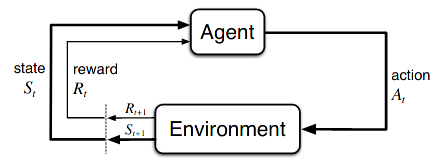
\includegraphics[width=0.6\linewidth]{figs/RL.png}
	\centering
	\caption{Interação agente-ambiente em um MDP \cite{sutton2018reinforcement}.} % figure 3.1 page 48
	\label{fig:mdp_env}
\end{figure}

Assim, dado um espaço de estados $\mathcal{S}$, um espaço de ações $\mathcal{A}$ e um espaço de recompensas $\mathcal{R}$, para cada par $(S, A)$ com $S \in \mathcal{S}$ sendo o estado atual do processo e $A \in \mathcal{A}$ a ação tomada pelo agente existe uma determinada probabilidade de atingir o estado $S' \in \mathcal{S}$ e receber a recompensa $R \in \mathcal{R}$ \cite{sutton2018reinforcement}.

Essa abordagem é bastante flexível e torna possível modelar a dinâmica do futebol virtual de robôs de diversas maneiras de modo que cada agente possa construir um estado percebido a partir de seus sensores e tomar decisões acerca de qual a melhor ação a fim de maximizar a recompensa recebida.

\subsection{MDP Episódico e Contínuo}

Um MDP pode ser caracterizado quanto à presença de um estado terminal. Caso o MDP tenha um ou mais estados que determinem o fim do processo, ele é dito episódico e a totalidade do processo até o estado que determina o fim é chamada de episódio. A simulação de futebol de robôs tratada neste trabalho é um exemplo de MDP episódico, uma vez que o MDP termina ao se encerrar o tempo de jogo.

Em contrapartida, há MDPs onde não está bem definido nenhum estado terminal. Nesses casos, o MDP pode continuar indefinidamente até que uma ação externa ao MDP determine a sua parada. Um exemplo disso é um MDP que controle um robô numa linha de produção. Caso o sistema de automação supervisor desse robô não determine sua parada (por falta de insumos, por exemplo), o MDP pode seguir operando indefinidamente.

% Nesta fundamentação, será tratado com mais atenção o caso episódico uma vez que é o caso que interessa para aplicação na simulação de futebol de robôs.
% (comentei fora essa parte porque a gente acabou fazendo o algoritmo contínuo usando o gamma lá porque a gente não codificou o tempo de jogo no estado)

\subsection{Recompensa e Retorno}

Como definido acima, para cada ação tomada em um MDP é atribuída uma recompensa $R \in \mathcal{R}$. Essa recompensa é sempre referente ao instante de tempo anterior, ou seja, não depende de qualquer outro fator que não o par $(S_t, A_t)$ executados no instante $t$ e a função de probabilidade associada pelo MDP a esse par. Por isso, é comum utilizar a notação $R_{t+1}$ para se referir à recompensa obtida após tomar a ação $A_t$ no instante de tempo $t$.

Porém em muitos casos é esperado de um agente que ele tome decisões que maximizem a recompensa total a longo prazo, ou seja, em um MDP episódico é esperado que se escolha $A_t$ a fim de maximizar não apenas $R_{t+1}$ mas sim o retorno $G_{t}$ tal que:

\begin{equation}
G_{t} = R_{t+1} + R_{t+2} + \dotsc + R_{terminal}.
\end{equation}

Caso o MDP seja contínuo, $G_t$ poderia divergir, uma vez que seja uma soma infinita de parcelas. Para solucionar o problema, basta adicionar à equação um fator de desconto ($\gamma$), tal que seja possível ajustar a relevância de recompensas futuras para o cálculo do retorno:

\begin{equation}
	G_{t} = R_{t+1} + \gamma R_{t+2} + \gamma^2 R_{t+3} + \dotsc = \sum_{k=1}^{\infty} \gamma^k R_{t+k+1}.
\end{equation}
% 
Observa-se que, para $ 0 \leq \gamma < 1$, o somatório converge. Para $\gamma = 0$, o retorno leva em consideração apenas a recompensa imediata $R_{t+1}$. Em contrapartida, para $\gamma \to 1$, as recompensas mais distantes no futuro são cada vez menos descontadas, ou seja, o agente tende a levar mais em consideração os ganhos futuros.

\subsection{Políticas e Funções de Valor}

É dado o nome de política para qualquer função $\pi: (S, A) \to \mathbb{R}$ que associe um estado qualquer do MDP e uma ação a uma probabilidade de se tomar essa ação diante desse estado, ou seja, $\pi(A|S) = p$ onde $p$ é a probabilidade de selecionar a ação A diante do estado S.

Para cada política $\pi$ existe uma função $v_\pi: (S) \to \mathbb{R}$ que, para cada estado, define a esperança de retorno caso o agente continue seguindo a política $\pi$. A função $v_\pi$ é conhecida como função de valor sob a política $\pi$.

Similarmente, existe uma função $q_\pi: (S, A) \to \mathbb{R}$ que, para cada par de estado e ação, define a esperança de retorno. Neste caso, a função $q_\pi$ é conhecida como função de valor da ação sob a política $\pi$.

É possível comparar duas políticas $\pi$ e $\pi'$ a respeito de suas funções $q$. A política $\pi$ é considerada melhor ou igual a $\pi$, ou $\pi \ge \pi'$, caso $q_\pi(S, A) \ge q_{\pi'}(S, A)$ para todo par $(S, A)$.

Sempre há ao menos uma política melhor ou igual a todas as outras, denominada política ótima. Qualquer política que cumpra esse requisito é denominada $\pi_*$ e, caso haja mais de uma, todas devem possuir a mesma função $q$ denominada $q_*$ \cite{sutton2018reinforcement}. No decorrer deste trabalho serão utilizadas técnicas que buscam estimar $q_*$. % chap 3.6 

Uma política que toma sempre o caminho de maior retorno é denominada gulosa e uma política que toma o caminho de maior retorno mas escolhe uma ação aleatoriamente com probabilidade parametrizada $\epsilon$ é denominada $\epsilon$-gulosa.


\section{Aprendizagem por Reforço}

Dada uma modelagem do problema como um MDP, resta obter uma maneira de estimar as probabilidades que determinam a dinâmica desse MDP para determinar a política capaz de maximizar a recompensa a longo prazo recebida pelo agente. O conjunto de técnicas que resolvem esse tipo de problema é chamado de Aprendizagem por Reforço.

No campo da aprendizagem de máquina, ela se difere da Aprendizagem Supervisionada por não haver um conjunto de pares $(s, a)$ considerados como verdade fundamental.
Nesse tipo de aprendizagem, o objetivo é extrapolar uma solução genérica a partir de exemplos de um conjunto de treinamento dado como correto, o que não é prático em problemas em que não se tem exemplos de comportamentos esperados e que representem bem o conjunto total de situações possíveis.
Ela também se diferencia da Aprendizagem Não-Supervisionada, que tradicionalmente visa encontrar estrutura em conjuntos de dados não classificados, enquanto a Aprendizagem por Reforço visa maximizar um sinal de recompensa \cite{sutton2018reinforcement}.

Desse modo, as técnicas de Aprendizagem por Reforço serão aplicadas a fim de buscar políticas capazes de maximizar o desempenho dos jogadores virtuais, ou seja, obter políticas que tornem os agentes capazes de fazer gols e evitar que os jogadores do time adversário façam gols.

\subsection{Aprendizagem com Diferença Temporal}
\par A aprendizagem com diferença temporal (\textit{temporal-difference learning}, ou TD) é uma das ideias centrais de RL \cite{sutton2018reinforcement}. Esse tipo de aprendizado é importante pois permite o aprendizado sem um modelo prévio do MDP do ambiente e também permite o uso de estimativas aprendidas durante o treinamento, conhecido como \textit{bootstrapping}, acelerando dramaticamente o tempo de convergência. 
\par A diferença temporal se apoia na ideia de que a política aproximada e a função de valor devem se relacionar de forma que ambas convirjam para seus valores ótimos, conhecida como iteração generalizada da política (\textit{generalized policy iteration} ou GPI) \cite{sutton2018reinforcement}. 
\par As técnicas \textit{Sarsa}, \textit{Q-learning} e \textit{Double Q-learning} apresentadas nas Subseções \ref{subsec:sarsa-theory}, \ref{subsec:q-theory} e \ref{subsec:dq-theory} são exemplos de aprendizagem com diferença temporal.

\subsection{Aprendizagem On-policy e Off-policy}
\label{subsec:on-off-policy}
Entre as técnicas de aprendizagem por reforço existe uma divisão entre a aprendizagem on-policy e a aprendizagem off-policy, referentes à relação entre a política executada durante o aprendizado e a política sobre a qual se quer aprender.

Nos algoritmos de aprendizagem on-policy o agente aprende a respeito da política $\pi$ enquanto navega o MDP de acordo com a própria política $\pi$, ou seja, a política executada durante a aprendizagem é a mesma que se quer estudar.

Em contrapartida, nos algoritmos de aprendizagem off-policy o agente aprende a respeito da política alvo $\pi$ enquanto navega o MDP de acordo com a política $b$, ou seja, ele estima a função $q_{\pi}$ enquanto executa a política $b$. Esses métodos costumam introduzir variância no processo, tornando o aprendizado ruidoso e muitas vezes divergente.

Além disso, é possível observar que a aprendizagem on-policy é apenas um caso particular da aprendizagem off-policy em que $b = \pi$.

\subsection{Soluções Tabulares e Aproximadas}

A maioria dos métodos de aprendizagem por reforço são testados e validados em MDPs cujos espaços de estados $\mathcal{S}$ e de ações $\mathcal{A}$ são suficientemente pequenos. Para esses MDPs é possível utilizar uma solução tabular, ou seja, a função $Q$ poda ser armazenada em uma tabela de tamanho razoável e sua imagem para cada par estado-ação pode ser atualizado individualmente.

Infelizmente em diversas aplicações a quantidade de estados possíveis é grande demais ou até mesmo infinita, como é o caso de sistemas em que determinada característica do estado é medida como uma grandeza contínua. Nesses casos, é impossível esperar que se obtenha soluções ótimas mesmo com tempo infinito, portanto o objetivo é obter uma solução aproximada que seja boa o suficiente para a aplicação desejada.

A ferramenta matemática utilizada para viabilizar soluções aproximadas é o conceito de aproximadores de função, muito utilizados na aprendizagem supervisionada. Entre os aproximadores mais utilizados estão os aproximadores lineares e as redes neurais multicamada.

\subsection{A Tríade da Morte}

Sutton e Barto definem um cenário denominado a tríade da morte (\textit{the deadly triad}) como um cenário onde a presença de três elementos causa instabilidade e divergência em treinamentos: aproximação de funções, \textit{bootstrapping} e treinamentos off-policy \cite{sutton2018reinforcement}.

Existe, portanto, a decisão do projetista de definir treinamentos de forma a evitar o conjunto desses três elementos. O aproximador de funções pode ser evitado com técnicas tabulares em ambientes menos complexos e ao custo de uso de memória. Para métodos TD, \textit{bootstrapping} é um requerimento. Entretanto, outros métodos permitem realizar o treinamento sem o uso de estimativas. Métodos off-policy são considerados mais poderosos e versáteis porém introduzem mais variância como descrito na Subseção \ref{subsec:on-off-policy} portanto nem sempre são a melhor escolha.

\subsection{Sarsa}
\label{subsec:sarsa-theory}
Entre os algoritmos de aprendizagem on-policy está o Sarsa. Seu nome é derivado da quíntupla $(S_t, A_t, R_{t+1}, S_{t+1}, A_{t+1})$ utilizada como entrada da sua fórmula de atualização:

\begin{equation}
	Q(S_t, A_t) \leftarrow Q(S_t, A_t) + \alpha[R_{t+1} + \gamma Q(S_{t+1}, A_{t+1}) - Q(S_t, A_t)].
\end{equation}

Uma vez que a política adotada pelo agente não pode ser gulosa, uma vez que ela inibiria a exploração do espaço de estados e de ações, é interessante que o agente siga uma política $\epsilon$-gulosa baseada na estimativa de $Q$. Nesse caso, para Q tabular, a convergência para a política ótima é garantida desde que todos os pares $(S, A)$ sejam visitados infinitas vezes e a política convirja para a política gulosa em $t \to \infty$.

Para o caso em que se usa um aproximador para estimar Q não há garantias, porém a natureza on-policy do Sarsa reduz a variância da aprendizagem. Isso pode tornar essa abordagem mais estável do que o Q-learning, descrito a seguir.

\subsection{Q-Learning}
\label{subsec:q-theory}
Um dos algoritmos mais populares no campo da aprendizagem por reforço é o Q-Learning. Trata-se de um método off-policy que aproxima diretamente a função $q_*$ independente da política que estiver sendo adotada pelo agente durante o treinamento.

O algoritmo é também muito simples. Dada uma representação tabular $Q: (\mathcal{S},\mathcal{A}) \to \mathbb{R}$ da função $q_*$, para cada instante de tempo $t$ é realizada a seguinte atualização a fim de aproximar $Q$ de $q_*$:

\begin{equation}
Q(S_t, A_t) \leftarrow Q(S_t, A_t) + \alpha[R_{t+1} + \gamma\max_{a} Q(S_{t+1}, a) - Q(S_t, A_t)],
\end{equation}
% 
sendo $\alpha$ o fator de aprendizagem, responsável por suavizar o impacto de cada atualização da tabela, e $\gamma$ o fator de desconto, responsável por reduzir a relevância de recompensas muito distantes no tempo.

Após iterações suficientes, espera-se que $Q$ convirja para $q_*$. Em certas condições a convergência é matematicamente garantida.

Uma vez estimada a função $q_*$, é simples obter a política ótima. Basta escolher a ação que maximiza $q_*$ no estado atual, ou seja:

\begin{equation}
A_{t} = \max_{a} q_*(S_t, a).
\end{equation}

É comum, mas não obrigatório, que a política $b$ seguida durante o aprendizado seja $epsilon$-gulosa em relação à aproximação $Q$.

\subsection{Q-Learning Duplo}
\label{subsec:dq-theory}
Apesar de popular o Q-Learning possui um problema de viés de maximização. Uma vez que a aproximação $Q$ é imprecisa no início do treinamento, é possível que o retorno esperado estimado seja enviesado para um valor maior do que o real.

Como solução para esse problema é utilizada a abordagem do Q-Learning Duplo. Nela são utilizadas duas aproximações, $Q_1$ e $Q_2$, e a atualização de $Q$ é dada da seguinte forma:

\begin{equation}
\label{eq:doubleq}
Q_1(S_t, A_t) \leftarrow Q_1(S_t, A_t) + \alpha[R_{t+1} + Q_2(S_{t+1}, \text{arg}\max_a Q_1(S_{t+1}, a)) - Q_1(S_t, A_t)].
\end{equation}
% 
Em metade das iterações (através de um sorteio, por exemplo), as aproximações $Q_1$ e $Q_2$ são trocadas. Com isso é anulado o viés de maximização gerado pelo uso de $\max_a Q$ como estimativa de retorno para os estados seguintes.

Outra vantagem desse método é que apesar de dobrar os requisitos de memória do algoritmo, afinal será preciso armazenar os dados referentes a duas aproximações, ele não aumenta o custo computacional por iteração.
